%======================================================================
% GMI-01 Topologicke variety.pdf
%======================================================================
\section{Topologické prostory a variety}
\strana{GMI-01-1}

\begin{itemize}[nosep]
  \item Topologické prostory
  \item Charakteristiky topologických prostorů
  \item Topologická varieta
  \item Klasifikace topologických variet
\end{itemize}

%----------------------------------------------------------------------
\strana{GMI-01-2}
\subsection{Topologické prostory}

\begin{definice}[Topologický prostor]
\kw{topologický prostor} $(X,\mathcal{T}) \equiv$
\begin{itemize}[nosep]
  \item[] $X$ \quad podkladový prostor
  \item[] $\mathcal{T}$ \quad soubor podmnožin $X$ splňující: \hfill (otevř.\ množ.)
  \begin{itemize}[nosep]
    \item $\emptyset, X\in\mathcal{T}$
    \item libovolné sjedn.\ množ.\ z $\mathcal{T}$ patří do $\mathcal{T}$
    \item libov.\ konečný průnik mn.\ z $\mathcal{T}$ patří do $\mathcal{T}$
  \end{itemize}
\end{itemize}
$\mathcal{T}$ nazýváme \kw{topologií} prostoru $X$, \\
množiny z $\mathcal{T}$ nazýváme \kw{otevřené mn.} \\
místo $(X,\mathcal{T})$ píšeme jen $X$
\end{definice}

\begin{vysvetleni}[Proč topologie]
Topologie je minimální struktura, která umožňuje mluvit o \uv{blízkosti} bodů, okolích, konvergenci a spojitosti, aniž bychom potřebovali vzdálenost. \uv{Okolí bodu $x$} znamená (otevřenou) množinu z $\mathcal{T}$ obsahující $x$. Axiomy kopírují vlastnosti otevřených množin v $\mathbb{R}^n$: sjednocení libovolně mnoha otevřených je otevřené, ale průnik jen konečně mnoha (např.\ $\bigcap_{k}(-\tfrac1k,\tfrac1k)=\{0\}$ už otevřené není). Varieta bude v první řadě topologický prostor; diferenciální struktura (GMI-02) se přidá až nad ním. Krtouš (odd.~2.1) topologickou část jen předpokládá a odkazuje na standardní učebnice.
\end{vysvetleni}

\begin{definice}
\begin{tabular}{@{}ll}
\kw{otevř.\ mn.} & je množina z $\mathcal{T}$ \\
\kw{uzavř.\ mn.} & je komplement otevřené v $X$ \\
\kw{komponenta} & je mn., která je ot.\ i uzavř.\ a nelze \\
 & napsat jako disjunkt.\ sjedn.\ dvou takových \\
\kw{báze topologie} & je soubor otevř.\ mn., které pomocí \\
 & sjednocení a kon.\ průniků generuje celou topolog. \\
\kw{kompaktní mn.}: & každé pokrytí otevř.\ množinami obsahuje \\
 & konečné podpokrytí otevř.\ množ. \hfill ?
\end{tabular}
\end{definice}

\begin{vysvetleni}[Komponenta, báze, kompaktnost]
\begin{itemize}[nosep]
  \item Komponenta: (neprázdná) množina zároveň otevřená i uzavřená, kterou už nelze dál rozdělit na dvě neprázdné disjunktní takové množiny. Prostor je \emph{souvislý}, pokud jeho jedinými otevřeno-uzavřenými podmnožinami jsou $\emptyset$ a $X$. Pro lokálně souvislé prostory (např.\ variety) jsou to právě souvislé komponenty.
  \item Báze: stačí znát \uv{malé} otevřené množiny (např.\ koule), ostatní dostaneme jako jejich sjednocení.
  \item Kompaktnost je topologická náhrada \uv{konečnosti}; definice v poznámkách je standardní (otazník je z originálu). V $\mathbb{R}^n$ platí Heineho--Borelova věta: kompaktní $\Leftrightarrow$ uzavřená a omezená. Např.\ $S^n$ je kompaktní, $\mathbb{R}^n$ ani $(0,1)$ ne.
\end{itemize}
\end{vysvetleni}

\begin{definice}[Spojité zobrazení]
\kw{spojité zobrazení} mezi top.\ pr.\ $X$ a $Y$ $\equiv$ \quad $f: X\to Y$ \\
\quad $\forall x\in X\ \ \forall$ okolí $V\subset Y$ bodu $f(x)$ $\exists$ okolí $U$ bodu $x$ tak, že $f(U)\subset V$
\end{definice}

\begin{definice}[Homeomorfismus]
$\phi$ je \kw{homeomorf.} $\equiv$ 1-1 zobrazení, \ $\phi$ a $\phi^{-1}$ spojité
\end{definice}

\begin{vysvetleni}[Spojitost a homeomorfismus]
Definice spojitosti je zobecněním \uv{$\varepsilon$--$\delta$} definice: koule nahrazují obecná okolí. Ekvivalentně: $f$ je spojité $\Leftrightarrow$ vzor každé otevřené množiny je otevřený, $f^{-1}(V)\in\mathcal{T}_X$ pro $V\in\mathcal{T}_Y$.
Homeomorfismus (\uv{1-1} zde znamená bijekce) je izomorfismus topologických prostorů -- homeomorfní prostory jsou z hlediska topologie nerozlišitelné. Spojitost inverze je nutné žádat zvlášť: např.\ $t\mapsto(\cos t,\sin t)$ z $\langle 0,2\pi)$ na $S^1$ je spojitá bijekce, ale inverze není spojitá v bodě $(1,0)$.
\end{vysvetleni}

%----------------------------------------------------------------------
\strana{GMI-01-3}
\begin{priklad}[Př: metrické topologie]
metrický pr.\ s fcí vzd.\ $d(x,y)$ \\
báze topologie: koule libovolného polom.\ a středu
\[ B_{x_0}(r) = \{x,\ d(x,x_0) < r\} \]
různé metriky mohou generovat stejnou topol.
\end{priklad}

\begin{priklad}[Př: topologie na $\mathbb{R}^n$]
metrická topologie metriky $d = \sqrt{\Delta x_1^2 + \Delta x_2^2 + \dots}$ \\
(v libovolných souř.)
\end{priklad}

\begin{priklad}[Př: diskrétní topologie]
generovaná 1-prvkovými mn.\ $\{x\}$, \ $x\in M$
\end{priklad}

\begin{vysvetleni}[K příkladům]
\begin{itemize}[nosep]
  \item \uv{Stejnou topologii} generují např.\ všechny normy na $\mathbb{R}^n$ (euklidovská, $\max_i|\Delta x_i|$, $\sum_i|\Delta x_i|$): každá koule jedné metriky obsahuje kouli druhé se stejným středem.
  \item \uv{V libovolných souř.} znamená v libovolných kartézských (afinních) souřadnicích -- jiná volba dá jinou metriku, ale stejnou topologii.
  \item Diskrétní topologie: otevřená je \emph{každá} podmnožina. Je metrická, generuje ji $d(x,y)=1$ pro $x\neq y$. Spojité je pak každé zobrazení z ní.
\end{itemize}
\end{vysvetleni}

%----------------------------------------------------------------------
\strana{GMI-01-4}
\subsection{Charakteristiky topologických prostorů}

\textbf{podle separovatelnosti:}
\begin{itemize}
  \item \kw{Hausdorffův prostor} \quad (T2) \\
        každé dva body oddělitelné otevř.\ mn. \\
        \quad $\forall x,y\in M$ (různé) \ $\exists\, U,V\in\mathcal{T}$: \ $x\in U$, $y\in V$, $U\cap V = \emptyset$

        příklad neHausdorff.\ pr.: přímka s 2 počátky
        \begin{center}
        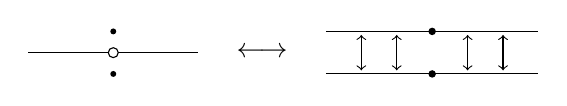
\begin{tikzpicture}[scale=0.9]
          \draw (0,0) -- (2.4,0);
          \draw[fill=white] (1.2,0) circle (2pt);
          \fill (1.2,0.3) circle (1.2pt);
          \fill (1.2,-0.3) circle (1.2pt);
          \node at (3.3,0) {$\longleftrightarrow$};
          \draw (4.2,0.3) -- (7.2,0.3);
          \draw (4.2,-0.3) -- (7.2,-0.3);
          \fill (5.7,0.3) circle (1.5pt);
          \fill (5.7,-0.3) circle (1.5pt);
          \foreach \x in {4.7,5.2,6.2,6.7} \draw[<->] (\x,0.25) -- (\x,-0.25);
        \end{tikzpicture}
        \end{center}
        platí: kompaktní disj.\ mn.\ jsou oddělitelné ot.\ mn.
  \item \kw{regulární Hausdorffův pr.} \quad (T3) $\equiv$ H + \\
        bod a uzavř.\ mn.\ mohou být odděleny ot.\ mn.
  \item \kw{normální Hausdorffův pr.} \quad (T4) $\equiv$ H + \\
        každé dvě disj.\ uzavř.\ mn.\ oddělitelné ot.\ mn.
\end{itemize}

\begin{vysvetleni}[Přímka se dvěma počátky]
Obrázek: vezmeme dvě kopie $\mathbb{R}$ a ztotožníme body $t\neq 0$ (svislé šipky), počátky $0_1, 0_2$ ztotožněny nejsou. Výsledek je lokálně euklidovský (každý bod má okolí homeomorfní intervalu) a má spočetnou bázi, ale každé okolí $0_1$ a každé okolí $0_2$ se protínají (obsahují body $t\neq0$ blízko nuly) -- prostor není Hausdorffův. Posloupnost $1/k$ v něm konverguje k \emph{oběma} počátkům. Proto se v definici variety Hausdorffovost explicitně požaduje: zaručuje jednoznačnost limit (a tedy např.\ jednoznačnost řešení diferenciálních rovnic na varietě).
\end{vysvetleni}

\textbf{podle \uv{velikosti} topologie}
\begin{itemize}
  \item \kw{prostor se spočetnou bází topologie} (second countable)
  \item \kw{parakompaktní pr.} \\
        každé otevřené pokrytí má lokálně konečné zjemnění \\
        lokálně konečné $\equiv$ $\forall x\ \exists$ okolí $V$ bodu $x$: $V$ protíná jen konečný počet množ.\ zjemněného pokrytí
  \item \kw{lokálně spočetný} (first countable) \\
        každý bod má spočetnou lokální bázi topologie
  \item \kw{Lindelöf.\ pr.} \\
        každé otevř.\ pokrytí má spočetné podpokrytí
  \item \kw{separabilní pr.} \\
        má spočetnou hustou podmnožinu
  \item \kw{kompaktní pr.} \\
        každé otevř.\ pokrytí má konečné podpokrytí
  \item \kw{lokálně kompaktní pr.} \\
        každý bod má kompaktní okolí
\end{itemize}

\begin{vysvetleni}[Parakompaktnost a spočetnost]
\emph{Zjemnění} pokrytí $\{U_\alpha\}$ je pokrytí $\{V_\beta\}$, kde každé $V_\beta$ leží v nějakém $U_\alpha$. Parakompaktnost je oslabení kompaktnosti: místo konečného podpokrytí stačí, aby se kolem každého bodu \uv{potkalo} jen konečně mnoho množin. To je přesně to, co je potřeba pro existenci \emph{rozkladu jednotky} (viz GMI-02, Technikality), a tím pro lepení lokálních konstrukcí (metrika, integrál) do globálních.
Příklad: $\mathbb{R}^n$ má spočetnou bázi (koule s racionálním středem a poloměrem), je separabilní ($\mathbb{Q}^n$ je hustá), Lindelöfův, parakompaktní a lokálně kompaktní, ale není kompaktní.
\emph{Lokální báze} v bodě $x$ je soubor okolí $x$ takový, že v každém okolí $x$ leží některé z nich (v metrickém prostoru např.\ koule $B_x(1/k)$).
\end{vysvetleni}

\begin{priklad}[Př: neparakompaktní pr.\ = \uv{dlouhá} polopřímka]
\uv{slepení} nespočetna intervalů $\langle 0,1)$ \\
$\langle 0,1)\times\omega_1$ + uspořádání $\to$ top.\ s bází danou intervaly \\
\quad ($\omega_1$ \dots\ první nespočetný ordinál)
\end{priklad}

\begin{vysvetleni}[Dlouhá polopřímka]
Body jsou dvojice $(t,\alpha)$, $t\in\langle 0,1)$, $\alpha<\omega_1$, uspořádané lexikograficky ($(t,\alpha)<(s,\beta)$, pokud $\alpha<\beta$, nebo $\alpha=\beta$ a $t<s$); topologie je dána otevřenými intervaly tohoto uspořádání. Klademe tedy za sebe nespočetně mnoho úseček. Prostor je Hausdorffův a lokálně euklidovský (kromě počátečního bodu, který je \uv{okrajový}; po odebrání $(0,0)$ jde o 1-dim.\ topologickou varietu), každý jeho počáteční úsek je homeomorfní intervalu -- ale je \uv{příliš dlouhý}: nemá spočetnou bázi, není parakompaktní ani metrizovatelný. Je to standardní protipříklad ukazující, že lokální euklidovskost + Hausdorff nestačí na \uv{rozumnou} varietu.
\end{vysvetleni}

%----------------------------------------------------------------------
\strana{GMI-01-5}
\textbf{\uv{celková slušnost} pr.}
\begin{itemize}
  \item \kw{lokálně euklidovský} dim.\ $n$ \\
        každý bod má otevř.\ okolí homeomorfní s oblastí v $\mathbb{R}^n$
  \item \kw{metrizovatelný} \\
        topologie generovaná metrikou (homeomorf.\ s metrick.\ p.)
  \item \kw{lokálně metrizovatelný} \\
        každý bod má metrizovatelné okolí
  \item \kw{kontrahovatelný pr.} \\
        prostor je homotopický bodu
  \item \kw{lokálně kontrahovatelný pr.} \\
        každý bod má kontrahovatelné okolí
\end{itemize}

\begin{vysvetleni}[Kontrahovatelnost]
\uv{Homotopický bodu} znamená homotopicky ekvivalentní jednobodovému prostoru: identitu na $X$ lze spojitě deformovat na konstantní zobrazení, $H:X\times\langle0,1\rangle\to X$, $H(\cdot,0)=\mathrm{id}$, $H(\cdot,1)=\text{konst}$. Např.\ $\mathbb{R}^n$ či koule jsou kontrahovatelné ($H(x,t)=(1-t)x$), $S^1$ není. Lokálně kontrahovatelný je každý lokálně euklidovský prostor (malé koule v mapě). Kontrahovatelnost oblastí je podstatná např.\ pro Poincarého lemma (uzavřená forma je lokálně exaktní).
\end{vysvetleni}

\begin{veta}[Vztahy mezi charakteristikami]
\begin{itemize}[nosep]
  \item T2 $\supset$ T3 $\supset$ T4
  \item kompaktní $\Rightarrow$ parakompaktní
  \item lokálně kompaktní $\wedge$ Hausdorff $\wedge$ spoč.\ báze top.\ $\Rightarrow$ parakompaktní
  \item metrizovatelný $\Rightarrow$ parakompaktní \quad (axiom výběru)
  \item metrizovatelný $\Leftrightarrow$ parakompaktní $\wedge$ Hausdorff $\wedge$ lok.\ metrizovat.
  \item regulární Hausdorf $\wedge$ spoč.\ báze top.\ $\Rightarrow$ metrizovatelný
  \item metriz.\ $\Rightarrow$ (kompaktní mn $\Leftrightarrow$ úplná a totálně omezená) \\
        \quad (tj.\ existuje konečné pokrytí oblastmi fixov.\ max velik.)
  \item metriz.\ $\Rightarrow$ (kompaktní mn $\Leftrightarrow$ každá posl.\ má konvergentní \\
        \quad podposloupnost s limitou v množině)
  \item parakompaktní Hausdorf $\Rightarrow$ normální Hausdorf
  \item parakompaktní Hausdorf $\Rightarrow$ exist.\ rozklad jednotky \\
        \quad podřízený libovolnému otevř.\ pokrytí
  \item spočetná báze top.\ $\Rightarrow$ lokálně spočetný \\
        spočetná báze top.
        $\left.\begin{array}{l}
          \Rightarrow \text{separabilní} \\
          \Rightarrow \text{Lindelöf}
        \end{array}\right\}$ \ pro metrizovatelné platí ekvivalence
\end{itemize}
\end{veta}

\begin{vysvetleni}[Jak číst vztahy]
\begin{itemize}[nosep]
  \item \uv{T2 $\supset$ T3 $\supset$ T4} je inkluze \emph{tříd} prostorů: každý normální Hausdorffův je regulární a ten je Hausdorffův (axiomy jsou čím dál silnější).
  \item Pojmenované věty: \uv{metrizovatelný $\Rightarrow$ parakompaktní} je Stoneova věta; \uv{$\Leftrightarrow$ parakompaktní + Hausdorff + lok.\ metrizovatelný} je Smirnovova metrizační věta; \uv{regulární Hausdorff + spočetná báze $\Rightarrow$ metrizovatelný} je Urysohnova metrizační věta; \uv{parakompaktní Hausdorff $\Rightarrow$ normální} je Dieudonnéova věta.
  \item \uv{Totálně omezená}: pro každé $\varepsilon>0$ existuje konečné pokrytí koulemi poloměru $\varepsilon$.
  \item Ekvivalence pro metrizovatelné prostory se týká jen separability a Lindelöfovosti: \emph{spočetná báze $\Leftrightarrow$ separabilní $\Leftrightarrow$ Lindelöf}. Lokální spočetnost (first countable) má \emph{každý} metrický prostor (koule $B_x(1/k)$), ale nespočetný diskrétní prostor spočetnou bázi nemá.
  \item Pro variety jsou nejdůležitější: Hausdorff + lokálně kompaktní + spočetná báze $\Rightarrow$ parakompaktní $\Rightarrow$ existují rozklady jednotky.
\end{itemize}
\end{vysvetleni}

%----------------------------------------------------------------------
\strana{GMI-01-6}
\subsection{Topologická varieta}

\begin{definice}[Topologická varieta]
\kw{topologická varieta} $M$ $\equiv$
\begin{itemize}[nosep]
  \item[] $M$ je lokálně euklidovský top.\ pr.
  \item[] $M$ je Hausdorffův
\end{itemize}
většinou se i uvažuje \\
\quad parakompaktní či \\
\quad se spoč.\ bází topologie \\
budeme uvádět explicitně
\end{definice}

\begin{vysvetleni}[Topologická varieta]
Varieta je prostor, který \uv{lokálně vypadá jako $\mathbb{R}^n$}: kolem každého bodu existuje okolí $U$ a homeomorfismus $x:U\to x(U)\subset\mathbb{R}^n$ na otevřenou množinu -- to je budoucí \emph{souřadnicová mapa} (GMI-02). Číslo $n$ je dimenze (na souvislé varietě je díky invarianci dimenze jednoznačná). Hausdorffovost vylučuje přímku se dvěma počátky, spočetná báze (resp.\ parakompaktnost) vylučuje dlouhou přímku a zaručuje rozklady jednotky, existenci riemannovské metriky a vnoření do $\mathbb{R}^N$. Příklady: $\mathbb{R}^n$, $S^n$, torus $T^n$, otevřené podmnožiny variet. Krtouš (odd.~2.1) definuje varietu rovnou jako topologický prostor s diferenciální strukturou danou atlasem; topologické předpoklady nerozebírá.
\end{vysvetleni}

\begin{veta}[pro topologické variety platí]
\begin{itemize}[nosep]
  \item top.\ varieta je disj.\ sjednocení souvislých komponent
  \item spočetná báze top.\ $\Rightarrow$ parakompaktnost
  \item parakompaktnost + spočetně komp.\ $\Rightarrow$ spočetná báze top.
  \item spočetná báze top.\ $\Leftrightarrow$ \oprava{separabilní}{separovatelný} a parakompaktní
  \item kompaktní $\Rightarrow$ spočetná báze top.
  \item metrizovatelný $\Leftrightarrow$ parakompaktní
  \item lokálně kompaktní
  \item lokálně souvislý
  \item lokálně spočetný
  \item lokálně kontrahovatelný
  \item lokálně metrizovatelný
\end{itemize}
\end{veta}

\begin{vysvetleni}[K vlastnostem variet]
\begin{itemize}[nosep]
  \item \uv{spočetně komp.} = \emph{spočetně mnoho komponent}: parakompaktní varieta má každou komponentu se spočetnou bází, celá varieta ji tedy má právě tehdy, když komponent je spočetně mnoho.
  \item V bodě \uv{spočetná báze $\Leftrightarrow$ \dots} jde o separabilitu (spočetnou hustou podmnožinu), ne o oddělitelnost bodů -- Hausdorffovost je v definici variety už zahrnuta a parakompaktní varieta s nespočetně mnoha komponentami (např.\ nespočetné disjunktní sjednocení přímek) spočetnou bázi nemá; separabilita vynutí spočetně mnoho komponent.
  \item \uv{metrizovatelný $\Leftrightarrow$ parakompaktní} plyne ze Smirnovovy věty: varieta je Hausdorffova a lokálně metrizovatelná (mapy přenesou metriku z $\mathbb{R}^n$).
  \item Lokální vlastnosti (poslední řádky) dědí varieta automaticky z $\mathbb{R}^n$ přes mapy.
\end{itemize}
\end{vysvetleni}

%----------------------------------------------------------------------
\strana{GMI-01-7}
\subsection{Klasifikace topologických variet}

\begin{tabular}{@{}l@{\quad}p{0.82\textwidth}}
$\dim = 0$ & diskrétní prostory -- pouze kardinalita (počet) \\[4pt]
$\dim = 1$ & parakompaktní souvislé homeomorfní $\mathbb{R}$ a $S^1$ \\
 & \phantom{parakompaktní} nesouvislé -- kombinace $\mathbb{R}$ a $S^1$ \\[4pt]
$\dim = 2$ & sféra \underline{s $g$ uchy}, případně \underline{s crosscapem} \\
 & \phantom{sféra s} {\small orientovatelné} \hspace{2.2cm} {\small neorientovatelné} \\[4pt]
$\dim = 3$ & úplná klasifikace založena na \kw{Thurstonově geometrizační hypotéze}: \\
 & \quad každou 3-varietu lze rozdělit na části s jednou z 8 typových (primárních) geometrií \\
 & dokázáno \\
 & \quad Thurston 1982 pro Hakenovy variety \\
 & \quad Grigori Perelman 2003 \\
 & \quad\quad (Ricci flow na bázi metody R.\ Hamiltona) \\
 & \quad\quad 2006 Fieldsova medaile \hfill (odmítl převzít) \\
 & \quad\quad 2010 Clay institut Millennium Prize za Poincarého hyp. \hfill (odmítl 1 mil \$) \\
 & implikuje platnost \kw{Poincarého hypotézy}
\end{tabular}

\begin{vysvetleni}[Klasifikace v dim.\ 1--3]
\begin{itemize}[nosep]
  \item dim 1: každá souvislá 1-varieta se spočetnou bází (bez okraje) je homeomorfní $\mathbb{R}$ (nekompaktní) nebo $S^1$ (kompaktní). Bez parakompaktnosti by přibyla dlouhá přímka.
  \item dim 2 (klasifikace \emph{kompaktních} souvislých ploch): orientovatelné jsou sféra s $g$ uchy (\uv{handles}; $g$ = rod; $g=0$ sféra, $g=1$ torus, \dots), neorientovatelné jsou sféra s $k\geq1$ crosscapy (vyříznutý kotouč nahrazen Möbiovým páskem; $k=1$ projektivní rovina $\mathbb{RP}^2$, $k=2$ Kleinova láhev).
  \item dim 3: osm Thurstonových geometrií je $S^3$, $E^3$, $H^3$, $S^2\times\mathbb{R}$, $H^2\times\mathbb{R}$, $\widetilde{SL}(2,\mathbb{R})$, Nil, Sol. Geometrizace tvrdí, že každou kompaktní orientovatelnou 3-varietu lze rozřezat podél sfér a torů na kusy nesoucí lokálně homogenní metriku jednoho z těchto typů. Perelmanův důkaz používá Ricciho tok $\partial_t g_{ab}=-2R_{ab}$ (s chirurgií).
\end{itemize}
\end{vysvetleni}

\begin{veta}[Poincarého hypotéza]
\begin{itemize}[nosep]
  \item jednoduše souvislá uzavřená 3-varieta je homeomorfní stand.\ sféře \\
        (neplatí pro $n > 3$)
  \item 3-varieta homotopicky ekvivalentní 3-sféře je homeomorfní stand.\ sféře \\
        (platí pro $n > 3$, ekvivalentní předchozímu pro $n = 3$)
\end{itemize}
\end{veta}

\begin{vysvetleni}[Poincarého hypotéza]
\emph{Uzavřená} = kompaktní bez okraje; \emph{jednoduše souvislá} = souvislá a každou uzavřenou křivku lze spojitě stáhnout do bodu ($\pi_1=0$). Pro $n>3$ první formulace neplatí: např.\ $S^2\times S^2$ je jednoduše souvislá uzavřená 4-varieta, která není sférou. Zobecněná (homotopická) verze platí ve všech dimenzích: $n\geq5$ Smale (1961), $n=4$ Freedman (1982), $n=3$ Perelman (2003). Pro 3-variety jsou formulace ekvivalentní, protože jednoduše souvislá uzavřená 3-varieta je už homotopicky ekvivalentní $S^3$.
\end{vysvetleni}

\begin{tabular}{@{}l@{\quad}p{0.82\textwidth}}
$\dim > 3$ & nemožná úplná klasifikace \\
 & rozhodnout, zda je prostor jednoduše souvislý, je nealgoritmický problém \\
 & jednoduše souvislé var.\ $\dim\geq 5$ lze klasifikovat
\end{tabular}

\begin{vysvetleni}[Proč nelze klasifikovat v dim.\ $\geq4$]
Každá konečně prezentovaná grupa je fundamentální grupou nějaké uzavřené 4-variety (a tedy i variety vyšší dimenze), a otázka, zda daná prezentace definuje triviální grupu, je algoritmicky nerozhodnutelná (Novikov--Boone). Proto neexistuje algoritmus rozhodující o jednoduché souvislosti, ani o homeomorfnosti variet (Markov 1958). Pro jednoduše souvislé variety dim.\ $\geq5$ tato překážka mizí a klasifikaci (např.\ pomocí teorie chirurgie) lze provést.
\end{vysvetleni}
